\clearpage
\begingroup
\section*{附录B：关键实验运行与验证记录}
\phantomsection
\addcontentsline{toc}{section}{附录B：关键实验运行与验证记录}
\titleformat{\subsection}{\zihao{4}\bfseries}{\thesubsection}{0.75em}{}
\renewcommand{\thesubsection}{B.\arabic{subsection}}
\renewcommand{\theHsubsection}{appendixB.\arabic{subsection}}
\setcounter{subsection}{0}

\subsection{SysY 三种实现的运行验证}
\label{app:sysy-records}
图片是命令输出与文件摘录的排版图，不是原生终端截图。原材料称部分内容来自 Ubuntu 20.04 对既有 ELF 的重新执行，但重跑脚本和日志未保留，不能核验该过程或称其重新编译。以下数值采用附录A所列 WSL2 Ubuntu 22.04 原实验核对。输入及独立预期位于 \path{tests/inputs/}，逐项记录位于 \path{artifacts/sysy/logs/}。

整数样例 \texttt{control\_matrix.initial\_full} 的三种实现均由 QEMU 执行，原 JSON 记录均为退出码 0，输出 \texttt{53 1 1 0 2}，与独立预期逐项相同。图\ref{fig:record-control}展示该样例，不能单独推出全部测试结论。
\begin{figure}[H]
\centering
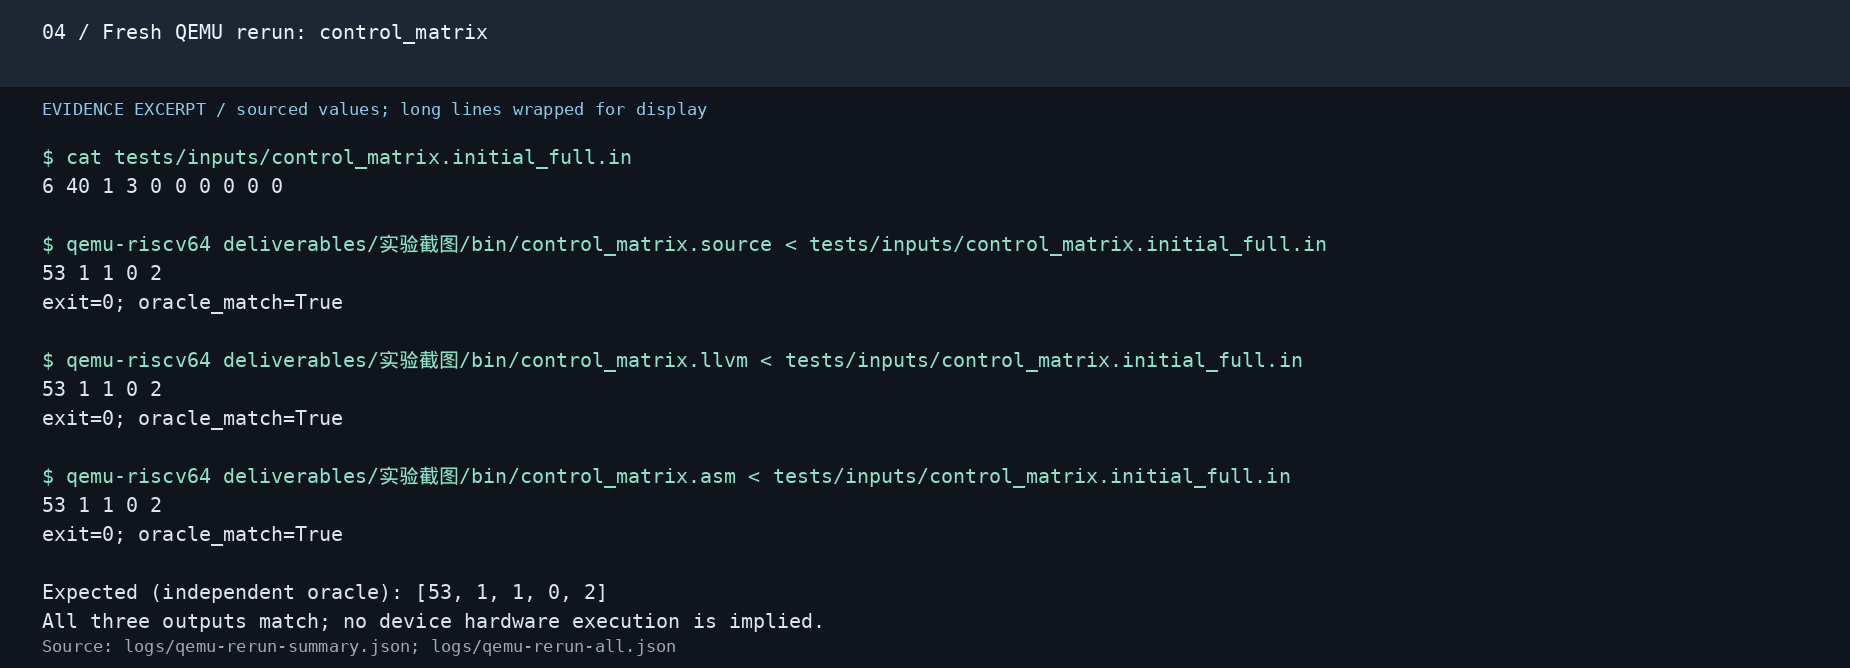
\includegraphics[width=\textwidth,keepaspectratio]{../materials/experiment-output/04-control_matrix-rerun.png}
\caption{整数示例三种实现的实验输出摘录。输入与输出可由原实验记录核对；图中异机重新执行的过程未单独核验。}
\label{fig:record-control}
\end{figure}

浮点样例 \path{float_stats.fractional} 的三种实现均输出三个值：\texttt{0x1.a7ae14p+1}、\texttt{3} 和 \texttt{0x1.a7ae14p-1}，对应数值约为 3.30999994、3 和 0.82749999，与独立 binary32 预期一致。十六进制文本是运行库输出格式，验证方法与第三章一致。
\begin{figure}[H]
\centering
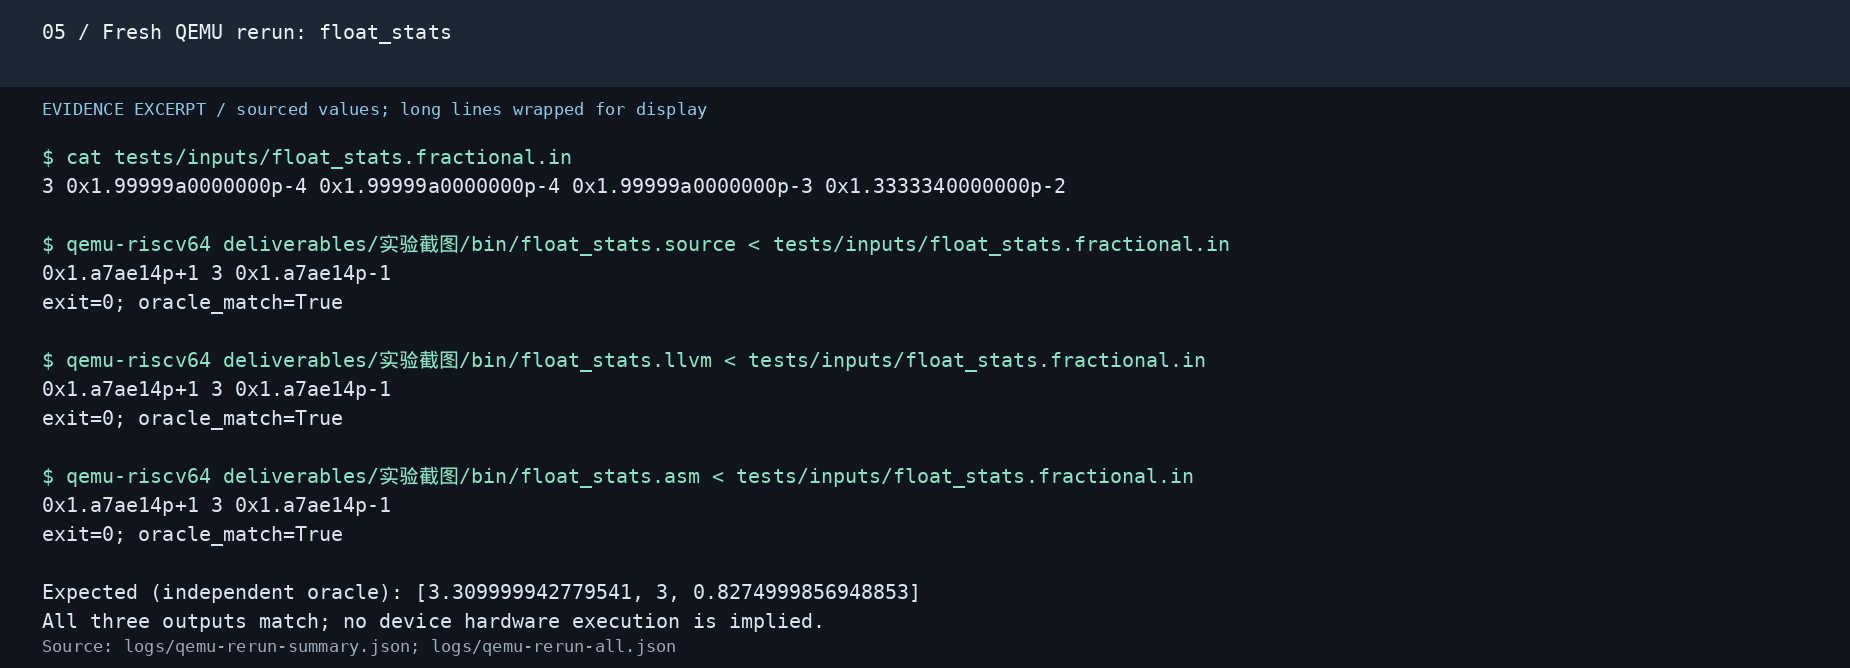
\includegraphics[width=\textwidth,keepaspectratio]{../materials/experiment-output/05-float_stats-rerun.png}
\caption{浮点示例三种实现的实验输出摘录。输出数值由原始日志与独立预期核对；图片保留原运行库输出格式。}
\label{fig:record-float}
\end{figure}

\clearpage
第三章的 480/480 结论依据 \path{artifacts/sysy/summary.json}、\path{artifacts/sysy/results.csv} 及 \path{artifacts/sysy/logs/} 中的完整记录：100 个整数用例与 60 个浮点用例分别执行三种实现，共 480 次，全部符合预期。图\ref{fig:record-summary}同时摘录原汇总和标为 2026-10-07 的重跑汇总；由于后者未附逐项原始记录，此处不将其计作另一轮已核验的 480 次执行，也不将两者相加。
\begin{figure}[H]
\centering
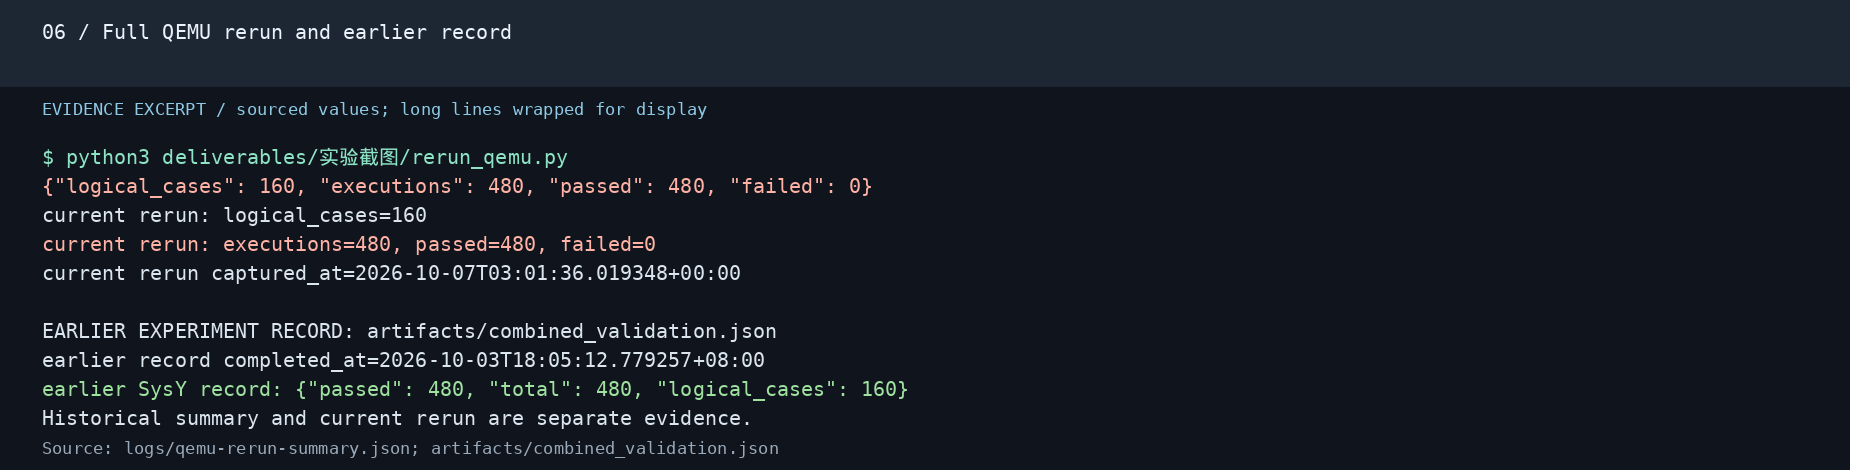
\includegraphics[width=\textwidth,keepaspectratio]{../materials/experiment-output/06-qemu-summary.png}
\caption{SysY 整体验证汇总摘录。正文采用有完整原始记录支持的 160 个用例、480 次执行；图中另列的历史重跑信息不扩大验证数量。}
\label{fig:record-summary}
\end{figure}

\subsection{AscendNPU IR 中端验证与后端限制}
\label{app:ascend-records}
图\ref{fig:record-backend}摘录六次主机侧处理、18/18 项 IR 核验及设备后端诊断。其结构与状态可由 \path{artifacts/mlir/verification-summary.json}、\path{artifacts/mlir/ascend-results.json} 和 \path{artifacts/mlir/06-full-compile.stderr.txt} 核对。图片中的工具缓存路径来自历史异机材料，不表示附录A所列 WSL 主机路径；本附录不据此认定该异机处理过程已独立复现。
\begin{figure}[H]
\centering
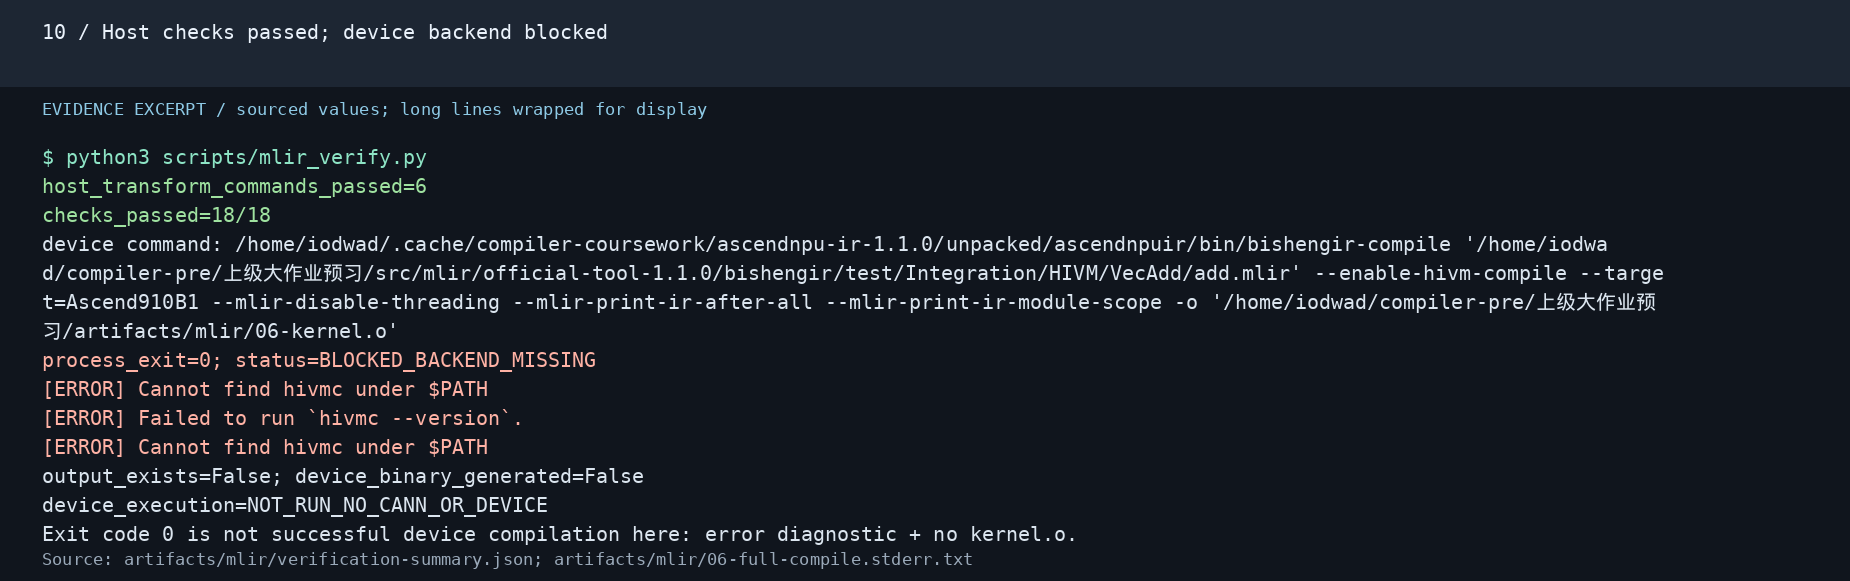
\includegraphics[width=\textwidth,keepaspectratio]{../materials/experiment-output/10-verification-and-backend.png}
\caption{AscendNPU IR 主机侧核验与设备后端限制的输出摘录。返回码 0 与缺少 hivmc 的错误同时存在，且没有生成设备目标文件。}
\label{fig:record-backend}
\end{figure}

已有结果验证的是主机上的中端变换、IR 重解析及指定结构。由于缺少 \texttt{hivmc}、CANN 与可用昇腾设备，尚未生成设备目标文件，也未在真实 Ascend 设备上进行数值或性能验证；主机侧检查通过不等于设备程序运行通过。第四章对 UB 布局、流水事件及模板调用的分析仍以相应完整 IR 为依据。
\endgroup
